\documentclass[aspectratio=169]{beamer}
\usetheme[titleformat=plain, % supported values: plain
          logo=i12en,        % supported values: i12en (default), i12de
          % itemsize=18pt,
          % defaultitemsep=0.4\baselineskip,
         ]{itc}

% Encoding and language
\usepackage[utf8]{inputenc}
\usepackage[T1]{fontenc}
\usepackage[english]{babel}
\usepackage{listings}
\usepackage{tikz}

% Meta information
\title{Title of Presentation}
\subtitle{Subtitle of Presentation}
\author{Til Mohr}
% Optional, appears on title page
\presenter{Til Mohr}
\institute{IT Center}
% \date{...} for a fixed date %TODO

\begin{document}


\begin{frame}[plain]
\titlepage
\end{frame}

\begin{frame}{Outline}
\tableofcontents
\end{frame}

\section{First topic}
\subsection{Itemize}
\begin{frame}{First topic}{Itemize}

\begin{itemize}
	\item Lorem ipsum dolor sit amet, consectetur adipiscing elit.
	\begin{itemize}
		\item Lorem ipsum dolor sit amet, consectetur adipiscing elit.
		\item Nunc porttitor odio a nisl placerat, nec suscipit ante dictum.
		\item Suspendisse venenatis nisl quis lectus molestie, et commodo sapien dapibus.
		\begin{itemize}
			\item Lorem ipsum dolor sit amet, consectetur adipiscing elit.
			\item Nunc porttitor odio a nisl placerat, nec suscipit ante dictum.
			\item Suspendisse venenatis nisl quis lectus molestie, et commodo sapien dapibus.
		\end{itemize}
	\end{itemize}
	\item Nunc porttitor odio a nisl placerat, nec suscipit ante dictum.
	\item Suspendisse venenatis nisl quis lectus molestie, et commodo sapien dapibus.
	\item Fusce quis tellus ac leo ornare viverra.
	\item Duis aliquam ex eget tortor ullamcorper porta.
\end{itemize}
\end{frame}

\begin{frame}[itemsep=1.25\baselineskip]{First topic}{Itemize with individual itemsep}
\begin{itemize}
	\item Lorem ipsum dolor sit amet, consectetur adipiscing elit.
	\item Nunc porttitor odio a nisl placerat, nec suscipit ante dictum.
	\item Suspendisse venenatis nisl quis lectus molestie, et commodo sapien dapibus.
	\item Fusce quis tellus ac leo ornare viverra.
	\item Duis aliquam ex eget tortor ullamcorper porta.
\end{itemize}
\end{frame}

\subsection{Enumerate}
\begin{frame}{First topic}{Enumerate}
\begin{enumerate}
\item First ...
\item ... Second
\begin{enumerate}
\item Nested
\begin{enumerate}
\item Another level
\end{enumerate}
\end{enumerate}
\end{enumerate}
\end{frame}

\section{Different Titles}
\begin{frame}
\sectionpage
\end{frame}

\begin{frame}{No subtitle}
\begin{itemize}
	\item Lorem ipsum dolor sit amet, consectetur adipiscing elit.
	\item Nunc eget lacus eget ante volutpat pulvinar eu sit amet diam.
	\item Cras nec magna sagittis, tempus ex id, condimentum lorem.
	\item Maecenas eget sem vel tellus posuere pellentesque nec ac sem.
\end{itemize}
\end{frame}

\begin{frame}{Empty subtitle}{}
\begin{itemize}
	\item Lorem ipsum dolor sit amet, consectetur adipiscing elit.
	\item Nunc eget lacus eget ante volutpat pulvinar eu sit amet diam.
	\item Cras nec magna sagittis, tempus ex id, condimentum lorem.
	\item Maecenas eget sem vel tellus posuere pellentesque nec ac sem.
\end{itemize}
\end{frame}


\lstdefinestyle{mycstyle}{
	language=C,
	breaklines=true,
	showstringspaces=false,
	keywordstyle=\color{blue}, 
	commentstyle=\color{green!50!black},
	escapeinside=||,
	basicstyle=\ttfamily,
	morecomment=[l][{\color{red!50!black}}]{\#},
	backgroundcolor=\color{black!4},
	numbers=left,
	numbersep=10pt,
	numberstyle=\footnotesize,
	framexleftmargin=0.1cm,
	xrightmargin=4.5cm, 
	xleftmargin=5cm,
	frame=lines,
	tabsize=4,
	belowskip=0cm,
}

\section{Misc}
\subsection{Listing}
\begin{frame}
\subsectionpage
\end{frame}

\begin{frame}[fragile]{Listing}
\vfill
\begin{lstlisting}[style=mycstyle, caption={Loop parallelization with OpenMP}]
#include <omp.h>

int main() {
#pragma omp parallel for
for (int i = 0; i < N; ++i) {
// some comment here
do_something();
}

return 0;
}
\end{lstlisting}
\vfill
\end{frame}

\begin{frame}{Test subtitle}{Lorem ipsum}
\begin{itemize}
\item Lorem ipsum dolor sit amet, consectetur adipiscing elit.
\item Nunc eget lacus eget ante volutpat pulvinar eu sit amet diam.
\item Cras nec magna sagittis, tempus ex id, condimentum lorem.
\item Maecenas eget sem vel tellus posuere pellentesque nec ac sem.
\item In mollis nunc at ipsum eleifend, et egestas elit volutpat.
\item Vivamus sed tellus malesuada, pretium sem ac, cursus mi.
\item Sed elementum sapien eget diam euismod laoreet.
\item Aliquam at magna sollicitudin nibh dignissim tincidunt.
\item Nunc ullamcorper turpis vel dui tempor, vitae scelerisque enim aliquam.
\item In ultricies augue suscipit velit interdum, a rutrum velit auctor.
\item Vivamus sed tellus malesuada, pretium sem ac, cursus mi.
\end{itemize}
\end{frame}

\begin{frame}{No subtitle}
\begin{itemize}
	\item Lorem ipsum dolor sit amet, consectetur adipiscing elit.
	\item Nunc eget lacus eget ante volutpat pulvinar eu sit amet diam.
	\item Cras nec magna sagittis, tempus ex id, condimentum lorem.
	\item Maecenas eget sem vel tellus posuere pellentesque nec ac sem.
	\item In mollis nunc at ipsum eleifend, et egestas elit volutpat.
	\item Vivamus sed tellus malesuada, pretium sem ac, cursus mi.
	\item Sed elementum sapien eget diam euismod laoreet.
	\item Aliquam at magna sollicitudin nibh dignissim tincidunt.
	\item Nunc ullamcorper turpis vel dui tempor, vitae scelerisque enim aliquam.
	\item In ultricies augue suscipit velit interdum, a rutrum velit auctor.
	\item Vivamus sed tellus malesuada, pretium sem ac, cursus mi.
	\item Sed elementum sapien eget diam euismod laoreet.
	\item Aliquam at magna sollicitudin nibh dignissim tincidunt.
\end{itemize}
\end{frame}

\begin{frame}{Figure Test}
\begin{figure}
	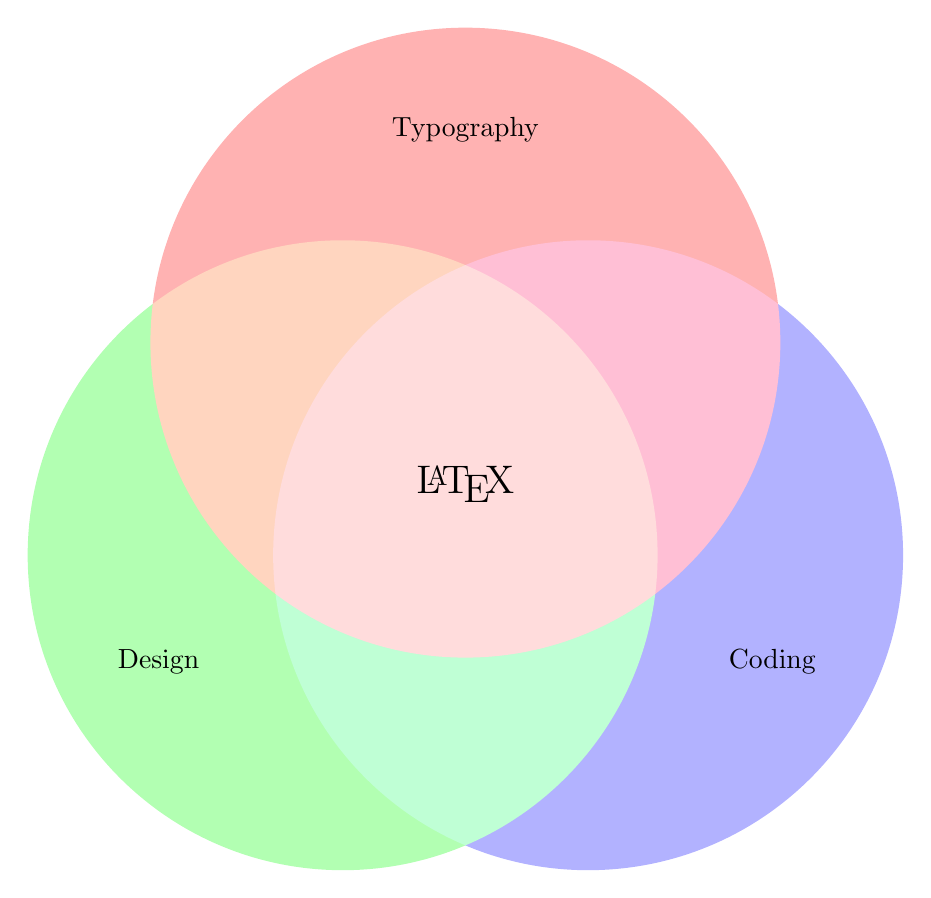
\begin{tikzpicture}
	\begin{scope}[blend group = soft light]
	\fill[red!30!white]   ( 90:1.8) circle (4);
	\fill[green!30!white] (210:1.8) circle (4);
	\fill[blue!30!white]  (330:1.8) circle (4);
	\end{scope}
	\node at ( 90:4.5)    {Typography};
	\node at ( 210:4.5)   {Design};
	\node at ( 330:4.5)   {Coding};
	\node [font=\Large] {\LaTeX};
	\end{tikzpicture}
	\caption{Test}
\end{figure}
\end{frame}

\begin{frame}{Block Test}
\begin{block}{Test}
This is a test block.
\end{block}
\vfill
\begin{definition}
This is a test definition.
\end{definition}
\vfill
\begin{theorem}
This is a test theorem.
\end{theorem}
\end{frame}

\end{document}
